\ifsvnmulti
 \svnkwsave{$RepoFile: siminos/lyapunov/QR.tex $}
 \svnidlong
 {$HeadURL$}
 {$LastChangedDate$}
 {$LastChangedRevision$} {$LastChangedBy$}
 \svnid{$Id$}
\fi

\renewcommand{\ssp}{x}            % state space point

\chapter{Co-moving frames}
\label{c:comoving}


\section{Frenet-Serret frames}
\label{sect:FrenSerr}

\textbf{Challenge:}
Describe here the Frenet-Serret  frames for both group orbits, and
the time-evolution orbit. Might find material from Lautrup\rf{Lau05},
Sect.~10.4 ``Mixed bending and twisting'' and Stone and
Goldbart\rf{StGo09} Exer.~12.10 useful. In particular, read up on the
Fermi-Walker frame used in monomode optical fibers, and the physical
significance of its rotation respective to the Frenet-Serret frame.

\SFIG{LautrupFrenetSerret}
{}{
The Frenet-Serret basis consists of the tangent vector $t$, the normal
$n$ and the binormal $b$. The normal points towards the center of
curvature $C$. As the point $x$ moves along the curve, the basis turns
around b and twists around $t$ to reflect the geometric curvature and
torsion of the oriented curve.
(from Lautrup\rf{Lau05})
}{}

Stone and Goldbart call the frame Serret-Frenet; which usage is right?
Lautrup says ``due to Frenet in 1847 (and independently to Serret in
1851)'', but Serret is more influential mathematician.
                                    \toCB
\emph{[Moved here from ChaosBook, return someday:]}
The eigenvalues and the eigen\-vectors of \stabmat\  ${\Mvar}_\stagn$
evaluated at a stagnation point $\ssp_\stagn$
\index{covariant Lyapunov vector}\index{Lyapunov!covariant vector}
\beq
{\Mvar}_\stagn \, \jEigvec[j](\ssp_\stagn)
   = \eigExp[j]_\stagn \,\jEigvec[j] (\ssp_\stagn)
\,,
\ee{cplxEigExp}
describe the linearized neighborhood of the \eqv\ point, with
$\eigExp[j]_p = \eigRe[j]_p \pm i\eigIm[j]_p$ and $\sign{p}^{(j)}$
independent of any particular coordinate choice.

\exercise{Constant Frenet-Serret  frames.}{\label{e-3-disk-symb}
\index{Frenet-Serret basis}
Prove that if both curvature and torsion are constants
independent of $s$, the curve becomes a perfect helix.
(Lautrup\rf{Lau05} Exer.~10.7)
} % end \exercise{Sensitivity to initial conditions}{

\begin{description}

\item[Predrag 2010-03-25 ]
Gilmore, Ginoux, Jones,
Letellier and Freitas\rf{GGJLF10}, \arXiv{1003.1703}
write: ``
The acceleration vector
\[
\gamma(t) = \frac{d \vel}{dt}
\]
is the time derivative of $\vel(t)$ at the instant $t$. The
chain rule leads to
\[
\gamma_j = \Mvar_{jk}\vel_k
\,.
\]
Gilmore \etal\ go beyond the zero-dimensional invariant sets of \eqva\
and introduce a {\em ``connecting''} curve that passes through  \eqva\ of
the autonomous dynamical system. The {\em ``connecting''} curve  can be
defined in two equivalent ways, (1) dynamically, as a ``vortex core''
curve through the eigenvalue-like equation
\(
\Mvar \, \vel = \Lyap  \, \vel
\,,
\)
and (2) kinematically, as the locus of points in the \statesp\ where the
principal curvature is zero.
''


\item[Predrag 2010-04-05 ]
\emph{From limit cycles to strange attractors}
by
William Ott and Mikko Stenlund,
\HREF{http://arxiv.org/abs/1004.0019}{arXiv:1004.0019}.
They say:
``
We define a quantitative notion of shear for limit cycles of flows. We
prove that strange attractors and SRB measures emerge when systems
exhibiting limit cycles with sufficient shear are subjected to periodic
pulsatile drives. The strange attractors possess a number of
precisely-defined dynamical properties that together imply chaos that is
both sustained in time and physically observable.
''

{\bf Predrag's 2010-04-05 notes:}
They require that $d\ssp/dt = \vel(\ssp)$ is $C^5$, start by looking at
an attractive cycle $p$ of length $L$ parametrized by length parameter
$s$, and let $\gamma : \reals \to \reals^d$ be a function of the
parameter $s$. The define $\Gamma = \{ \gamma(s) : s \in [0,L) \} $ and a
tubular neighborhood $\overline{\pS} =\Gamma \times D$, expressed in the
natural $(s,z )$-coordinates, where $D$ is a closed disk in
$\reals^{d-1}$1 of sufficiently small radius.

What might be of interest is the way they construct local normal basis by
applying the Gram-Schmidt procedure and utilizing the first $n$
derivatives $d^k\gamma(s)/ds^k$ to obtain is a skew-symmetric matrix of
generalized curvatures and identifying the co-moving differential
equation as the classical Frenet-Serret equation from differential
geometry.

\item[ES 2010-01-28]
Here is some stuff from Siminos thesis that might or might not be
relevant in this context:

Predrag dropped this but I am not sure: ``In general, when a \slice\
$\pSRed$ is defined through relations of the form $\overline{x}_i=0$,
$i=1,\ldots,N$ then we call $\pSRed$ a \emph{coordinate \slice}.''

Once a linear \slice\ $\pSRed=\{x_1=c_1,\ldots,x_r=c_N\}$ is defined by
the first $N$ coordinates (relabel coordinates as necessary), we write
the group transformations as
\beq
	\overline{x}= g \cdot x = w(g,x)\,.
	\label{eq:transNorm}
\eeq
Equating the first $N$ components of the function $w$ to the
constants in the definition of the {\slice} $\pSRed_i(x)=c_i$
yields the \emph{slice conditions} for $\pSRed$:
\beq
	\overline{x}_1=w_1(g,x)=c_1,\ldots,\overline{x}_N=w_N(g,x)=c_N\,.
	\label{eq:normalization}
\eeq
The slice conditions \refeq{eq:normalization} can always be
solved\rf{FelsOlver99} for the group parameters in terms of $x$, yielding
the moving frame associated with $\pSRed$: $\LieEl=\LieEl(x)$. For proof
\cf~\refrefs{FelsOlver98,FelsOlver99}. This can be thought of as
generalization of the Frenet-Serret co-moving frame.

\item[ES  2009-05-05]
Fels and Olver claim that ``a moving frame as an equivariant map from a
manifold to a Lie group'' is exactly \emph{their} interpretation of
\mframes\ so I've dropped this: The notion of a {\em moving frame} as a
map from a manifold to a Lie group was introduced by Cartan\rf{CartanMF}.

\end{description}


\section{Stability in a co-moving frame}
\label{sect:stabComoving}
% Predrag                           		2011-03-05
% moved to here halcrow/blog/TEX/QR.tex		2008-12-07

{\bf Predrag 2011-03-05}
{These appendices contain material that will eventually be returned back to
    ChaosBook.org. Please keep ChaosBook formatting throughout this chapter.
    Thanks!}

%%%%%%%%%%%%%%%%%%%%%%%%%%%%%%%%%%%%%%%%%%%%%%%%%%%%%%%%%%%%%%%%%%%%%%%%%%
\exercise{Stability in a co-moving frame.}{ \label{exer:stabComoving}
% Predrag                           19feb2008
\index{stability|co-moving frame}
\index{|co-moving frame|stability}
    %
\PC{ChaosBook: add this to Problems/exerAppApplic}
%
The {\em \stabmat}(velocity gradient matrix):
\index{matrix!stability}
\index{stability!matrix}
\index{velocity gradient matrix}
% % http://mathworld.wolfram.com/StabilityMatrix.html
% calls this `stability matrix'.
%   }
\beq
{\Mvar}_{ij}(\ssp) = \frac{\pde \vel_i(\ssp)}{\pde \ssp_j  }
\ee{appl:DerMatrix}
The linearized neighborhood is transported by the
{\jacobianM}
% This Jacobian matrix has inherited the name
% {\em fundamental solution matrix} or simply
% {\em fundamental matrix}
% from the theory of linear ODEs.
\index{fundamental matrix}
\beq
\jMps^t_{ij}(\xInit)
  =  \left. {\pde \ssp_i(t) \over \pde \ssp_j} \right|_{\ssp=\xInit}
\, .
\label{appl:hOdes}
\eeq
$\ExpaEig_k$ denotes
the $k$th
{\em eigen\-value}
(multiplier)
 of the finite time
 {\jacobianM} $\jMps^t$,
\index{stability!eigenvalue}
while $\eigExp[k]$ denotes
the $k$th {\em characteristic exponent}
or
{\em characteristic value},
% sometimes the same thing as the {\em Lyapunov exponent}),
with real part $\eigRe[k]$
% is sometimes the same thing as the {\em Lyapunov exponent}),
and phase $\eigIm[k]$:
\index{characteristic!exponent}
\index{characteristic!value}
% \index{Lyapunov exponent}
\beq
\ExpaEig_k
 =
e^{t \eigExp[k]}
 =
e^{t\eigRe[k] +i t\eigIm[k]}
\,.
\ee{appl:stabExpon}
$\derf{t}{\xInit}$ depends on the initial point $\xInit$
and the elapsed time $t$. For notational brevity we tend to
omit this dependence. Projection operator
\beq
{\PP}_i = \prod_{j\not= i}
   \frac{\jMps-\ExpaEig_j \matId }
        {\ExpaEig_i - \ExpaEig_j} \, ,
\ee{appl:stab:3.42}
projects arbitrary $\ssp \in \pS$ onto the $i$th eigenspace
of $\jMps$.

If you are evolving a high-dimensional flow with a handful of
expanding eigen-directions and contracting eigen-directions of
comparable magnitude, and the remaining many contracting eigen-directions
so contracting to be irrelevant. One would like to find a way to
economically evolve a local low-dimensional eigenvector frame of
$\jMps^t$ that keeps track only of these directions.

Initiate this construction by evaluating the leading
eigenvectors for a full-space $\jMps^T$ computed after the flow has
evolved for some typical turnover time $T$, and constructing
projection operators on this subspace by keeping in
\refeq{appl:stab:3.42} only $|\ExpaEig_i| > \ExpaEig_{min}$.

Now find {\em implementable} equations for $\ExpaEig_i$,
${\PP}_i$ time $t$ later.
Assume all relevant eigenvalues are distinct, and
the marginal (symmetry induced) eigenvalues have been eliminated.
If the projection operator notation
${\PP}_i$ is not to your taste, replace it
by left/right eigenvectors $\jEigvecT{i}$, $\jEigvec{j}$.

\begin{itemize}
\item[(a)]
    Show that the $j$th multiplier evolves in the co-moving frame as
\beq
\dot{\ExpaEig}_j = \Mvar_{jj} \ExpaEig_j
    \,,\quad
\Mvar_{jk}= {\PP}_j \Mvar {\PP}_k
    \,,\qquad \mbox{no sum on } j
\,.
\ee{appl:dotLambda}
\item[(b)]
    Show that the $j$th projection operator
    (or eigenvector) evolves as a set of ODEs
\beq
{\PP}_j \dot{\PP}_j  {\PP}_k = %\sum_{k \neq j}
            \frac{\ExpaEig_j}
                 {\ExpaEig_j - \ExpaEig_k} \Mvar_{jk}
    \,,\qquad k \neq j \mbox{, no sum on } j
\,.
\ee{appl:dotP}
\end{itemize}
These coupled ODEs are beguiling but useless for
hyperbolic flows, as $\ExpaEig_j$ contract/expand exponentially
with time, and projection operators become quickly uncomputable due to
numerical under/over flows. One needs to track instead the
finite time Lyapunov exponents
$
\eigExp[k](t) = (1/t) \ln \ExpaEig_k
$
which remain bounded for flows of bounded hyperbolicity.

\begin{itemize}
\item[(c)]
    Show that this is correct (or not):
\beq
\dot{\eigExp}^{(j)} = (\Mvar_{jj} - {\eigExp}^{(j)})/t
\,.
\ee{appl:dotlambda}
Explain the initial conditions.
Is there some smarter way of writing this (redefining time, whatever?)
\item[(d)]
    Write corresponding equations for ${\PP}_j$
    It is not clear that there is
    a sensible way - try keeping\rf{CV93,CBook:appendApplic}
    eigenvectors normalized
     $|\jEigvec{j}| = 1$?
\item[(e)]
    Deal with the complex eigenvalues case?
\item[(f)]
    Discuss likelihood that eigenvalues cross. What
happens to the eigenvectors?
\item[(g)]
    Test your formulation on Lorenz or R\"ossler.
\item[(h)]
    propose alternative, better co-moving frame methods?
\end{itemize}

\hfill Jean-Luc Thiffeault and Predrag Cvitanovi\'c
        }% end \exercise{Stability in a co-moving frame

\solution{exer:stabComoving}{Stability in a co-moving frame.}{
\index{stability|co-moving frame}
\index{|co-moving frame|stability}

See Dieci \etal\rf{DJRV07} on QR method (the paper is on
\HREF{http://www.math.ku.edu/~evanvleck/papers.html}
     {http://www.math.ku.edu/~evanvleck/papers.html})

The issue of projection operators becoming uncomputable due to
numerical under/over flows has been addressed
by Vattay and Cvitanovi\'c\rf{CV93,CBook:appendApplic}.

Recheck - is \refref{Thiffeault2001} or \refref{ThiBoo99} more relevant
here?

    } %end \exercise{Stability in a co-moving frame


\Remarks

\remark{Blah und Bluh.}{ \label{dscr:r:symmCycles}
We conclude with a few comments about
Lagrangian velocity gradient tensor turbulence averaging methods\rf{GLEM07}.
} %end \remark{Cycles and symmetries.}{


\section{Flow linearized about a hyperbolic equilibrium}


\begin{figure}
 % source in /dasbuch/book/FigSrc/inkscape/eqbHypbLin.svg
 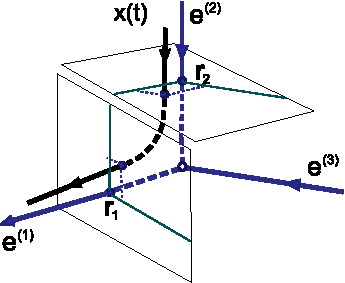
\includegraphics[width=0.45\textwidth]{eqbHypbLin}
  \caption{Linearization of a flow near to an equilibrium:
  the flow is reduced to an analytic map between two
  near Poincar\'e sections, mapping the in-flow into out-flow.
  }\label{f:eqbHypbLin}
\end{figure}
